\documentclass{article}\usepackage[]{graphicx}\usepackage[]{color}
%% maxwidth is the original width if it is less than linewidth
%% otherwise use linewidth (to make sure the graphics do not exceed the margin)
\makeatletter
\def\maxwidth{ %
  \ifdim\Gin@nat@width>\linewidth
    \linewidth
  \else
    \Gin@nat@width
  \fi
}
\makeatother

\definecolor{fgcolor}{rgb}{0.345, 0.345, 0.345}
\newcommand{\hlnum}[1]{\textcolor[rgb]{0.686,0.059,0.569}{#1}}%
\newcommand{\hlstr}[1]{\textcolor[rgb]{0.192,0.494,0.8}{#1}}%
\newcommand{\hlcom}[1]{\textcolor[rgb]{0.678,0.584,0.686}{\textit{#1}}}%
\newcommand{\hlopt}[1]{\textcolor[rgb]{0,0,0}{#1}}%
\newcommand{\hlstd}[1]{\textcolor[rgb]{0.345,0.345,0.345}{#1}}%
\newcommand{\hlkwa}[1]{\textcolor[rgb]{0.161,0.373,0.58}{\textbf{#1}}}%
\newcommand{\hlkwb}[1]{\textcolor[rgb]{0.69,0.353,0.396}{#1}}%
\newcommand{\hlkwc}[1]{\textcolor[rgb]{0.333,0.667,0.333}{#1}}%
\newcommand{\hlkwd}[1]{\textcolor[rgb]{0.737,0.353,0.396}{\textbf{#1}}}%
\let\hlipl\hlkwb

\usepackage{framed}
\makeatletter
\newenvironment{kframe}{%
 \def\at@end@of@kframe{}%
 \ifinner\ifhmode%
  \def\at@end@of@kframe{\end{minipage}}%
  \begin{minipage}{\columnwidth}%
 \fi\fi%
 \def\FrameCommand##1{\hskip\@totalleftmargin \hskip-\fboxsep
 \colorbox{shadecolor}{##1}\hskip-\fboxsep
     % There is no \\@totalrightmargin, so:
     \hskip-\linewidth \hskip-\@totalleftmargin \hskip\columnwidth}%
 \MakeFramed {\advance\hsize-\width
   \@totalleftmargin\z@ \linewidth\hsize
   \@setminipage}}%
 {\par\unskip\endMakeFramed%
 \at@end@of@kframe}
\makeatother

\definecolor{shadecolor}{rgb}{.97, .97, .97}
\definecolor{messagecolor}{rgb}{0, 0, 0}
\definecolor{warningcolor}{rgb}{1, 0, 1}
\definecolor{errorcolor}{rgb}{1, 0, 0}
\newenvironment{knitrout}{}{} % an empty environment to be redefined in TeX

\usepackage{alltt}
\usepackage[sc]{mathpazo}
\renewcommand{\sfdefault}{lmss}
\renewcommand{\ttdefault}{lmtt}
\usepackage[T1]{fontenc}
\usepackage{geometry}
\geometry{verbose,tmargin=2.5cm,bmargin=2.5cm,lmargin=2.5cm,rmargin=2.5cm}
\setcounter{secnumdepth}{2}
\setcounter{tocdepth}{2}
\usepackage[unicode=true,pdfusetitle,
 bookmarks=true,bookmarksnumbered=true,bookmarksopen=true,bookmarksopenlevel=2,
 breaklinks=false,pdfborder={0 0 1},backref=false,colorlinks=false]
 {hyperref}
\hypersetup{
 pdfstartview={XYZ null null 1}}

\makeatletter
%%%%%%%%%%%%%%%%%%%%%%%%%%%%%% User specified LaTeX commands.
\renewcommand{\textfraction}{0.05}
\renewcommand{\topfraction}{0.8}
\renewcommand{\bottomfraction}{0.8}
\renewcommand{\floatpagefraction}{0.75}

\makeatother
\IfFileExists{upquote.sty}{\usepackage{upquote}}{}
\begin{document}








The results below are generated from an R script.

\begin{knitrout}
\definecolor{shadecolor}{rgb}{0.969, 0.969, 0.969}\color{fgcolor}\begin{kframe}
\begin{alltt}
\hlcom{########################## Lab1 ##########################}
\hlcom{### Meta-info}
\hlcom{## Beta distribution}
\hlcom{## Simulations}
\hlcom{## Gini coefficient}
\hlcom{## Credible interval}
\hlcom{## Highest Posterior Density HPD}

\hlcom{# Task 1: Bernoulli ... again}
\hlcom{# a) Draw random numbers from Beta distribution and graphical verification}
\hlcom{# of posterior}
\hlcom{# b) Simulate to compute posterior prob of Pr(theta < 0.4)}
\hlcom{# c) Compute log-oods posterior distribution}

\hlcom{# Task 2: Log-normal distribution and the Gini coefficient}
\hlcom{# a) Simulate 1000 draws from posterior or theta2. Compare with real value}
\hlcom{# b) Compute posterior distribution of Gini coefficient G}
\hlcom{# c) Compute 95% equal tail credible interval of Gini coefficient G.}
\hlcom{# Doing a kernal density estimate}
\hlcom{# Compute 95% Highest Posterior Density interval (HPD) of G}

\hlcom{# Task 3: Bayesian inference for the concentration parameter in the von Mises distributio}
\hlcom{# a) Plot posterior distribution of kappa for wind direction data}
\hlcom{# b) Find approximate posterior mode of kappa}

\hlcom{############# Task 1 #############}
\hlcom{# Bernoulli ... again}
\hlcom{#a)}
\hlcom{# Instrucitons}
\hlcom{# Likelihood: y_1, ..., y_n | θ ~ Bern(θ)}
\hlcom{# Prior: θ ~ Beta(alpha_0, beta_0), alpha_0 = beta_0 = 2}
\hlcom{# Posterior: θ|y_1, ..., y_n ~ Beta(alpha_0 + s, beta_0 + f)}
\hlcom{# s = 14}
\hlcom{# n = 20}
\hlcom{# f = 6}

\hlcom{# Setup}
\hlstd{n} \hlkwb{=} \hlnum{20}
\hlstd{s} \hlkwb{=} \hlnum{14}
\hlstd{f} \hlkwb{=} \hlstd{n} \hlopt{-} \hlstd{s}
\hlstd{nDraws} \hlkwb{=} \hlnum{50000}
\hlstd{drawsInterval} \hlkwb{=} \hlnum{10}
\hlstd{intervalVec} \hlkwb{<-} \hlkwd{seq}\hlstd{(}\hlnum{10}\hlstd{, nDraws, drawsInterval)}

\hlcom{# Prior}
\hlstd{prior.alpha} \hlkwb{=} \hlnum{2}
\hlstd{prior.beta} \hlkwb{=} \hlnum{2}

\hlcom{# Posterior}
\hlstd{posterior.alpha} \hlkwb{<-} \hlstd{prior.alpha} \hlopt{+} \hlstd{s}
\hlstd{posterior.beta} \hlkwb{<-} \hlstd{prior.beta} \hlopt{+} \hlstd{f}
\hlstd{posterior.draws_means} \hlkwb{=} \hlkwd{numeric}\hlstd{()}
\hlstd{posterior.draws_sd} \hlkwb{=} \hlkwd{numeric}\hlstd{()}

\hlcom{# For-loop - (10, 20, 30, ..., 49980, 49990)}
\hlkwa{for} \hlstd{(i} \hlkwa{in} \hlstd{intervalVec) \{}
  \hlstd{posterior.draws} \hlkwb{<-} \hlkwd{rbeta}\hlstd{(}\hlkwc{n} \hlstd{= i,}
                           \hlkwc{shape1} \hlstd{= posterior.alpha,}
                           \hlkwc{shape2} \hlstd{= posterior.beta)} \hlcom{# Draw from beta}

  \hlstd{posterior.draws_means} \hlkwb{<-} \hlkwd{c}\hlstd{(posterior.draws_means,} \hlkwd{mean}\hlstd{(posterior.draws))} \hlcom{# Add mean to vector of means}
  \hlstd{posterior.draws_sd} \hlkwb{<-} \hlkwd{c}\hlstd{(posterior.draws_sd,} \hlkwd{sd}\hlstd{(posterior.draws))} \hlcom{# Add sd to vector of sd}
\hlstd{\}}

\hlcom{# True values}
\hlstd{posterior.true_mean} \hlkwb{<-} \hlstd{posterior.alpha}\hlopt{/}\hlstd{(posterior.alpha} \hlopt{+} \hlstd{posterior.beta)}
\hlstd{posterior.true_sd} \hlkwb{<-} \hlkwd{sqrt}\hlstd{((posterior.alpha}\hlopt{*}\hlstd{posterior.beta)}\hlopt{/}\hlstd{((posterior.alpha} \hlopt{+} \hlstd{posterior.beta)}\hlopt{^}\hlnum{2} \hlopt{*} \hlstd{(posterior.alpha} \hlopt{+} \hlstd{posterior.beta} \hlopt{+} \hlnum{1}\hlstd{)))}

\hlcom{# Plot}
\hlkwd{par}\hlstd{(}\hlkwc{mfrow} \hlstd{=} \hlkwd{c}\hlstd{(}\hlnum{1}\hlstd{,} \hlnum{2}\hlstd{))}
\hlkwd{plot}\hlstd{(}\hlkwc{x} \hlstd{= intervalVec,}
     \hlkwc{y} \hlstd{= posterior.draws_means,}
     \hlkwc{type} \hlstd{=} \hlstr{'l'}\hlstd{,}
     \hlkwc{xlab} \hlstd{=} \hlstr{'No. of draws'}\hlstd{,}
     \hlkwc{ylab} \hlstd{=} \hlstr{'Mean of data'}\hlstd{)} \hlcom{# Plot means}
\hlkwd{abline}\hlstd{(}\hlkwc{h} \hlstd{= posterior.true_mean,} \hlkwc{col} \hlstd{=} \hlstr{'red'}\hlstd{)} \hlcom{# Add line of real mean to plot}

\hlkwd{plot}\hlstd{(}\hlkwc{x} \hlstd{= intervalVec,}
     \hlkwc{y} \hlstd{= posterior.draws_sd,}
     \hlkwc{type} \hlstd{=} \hlstr{'l'}\hlstd{,}
     \hlkwc{xlab} \hlstd{=} \hlstr{'No. of draws'}\hlstd{,}
     \hlkwc{ylab} \hlstd{=} \hlstr{'Sd of data'}\hlstd{)} \hlcom{# Plot sd's}
\hlkwd{abline}\hlstd{(}\hlkwc{h} \hlstd{= posterior.true_sd,} \hlkwc{col} \hlstd{=} \hlstr{'red'}\hlstd{)}
\end{alltt}
\end{kframe}

{\centering 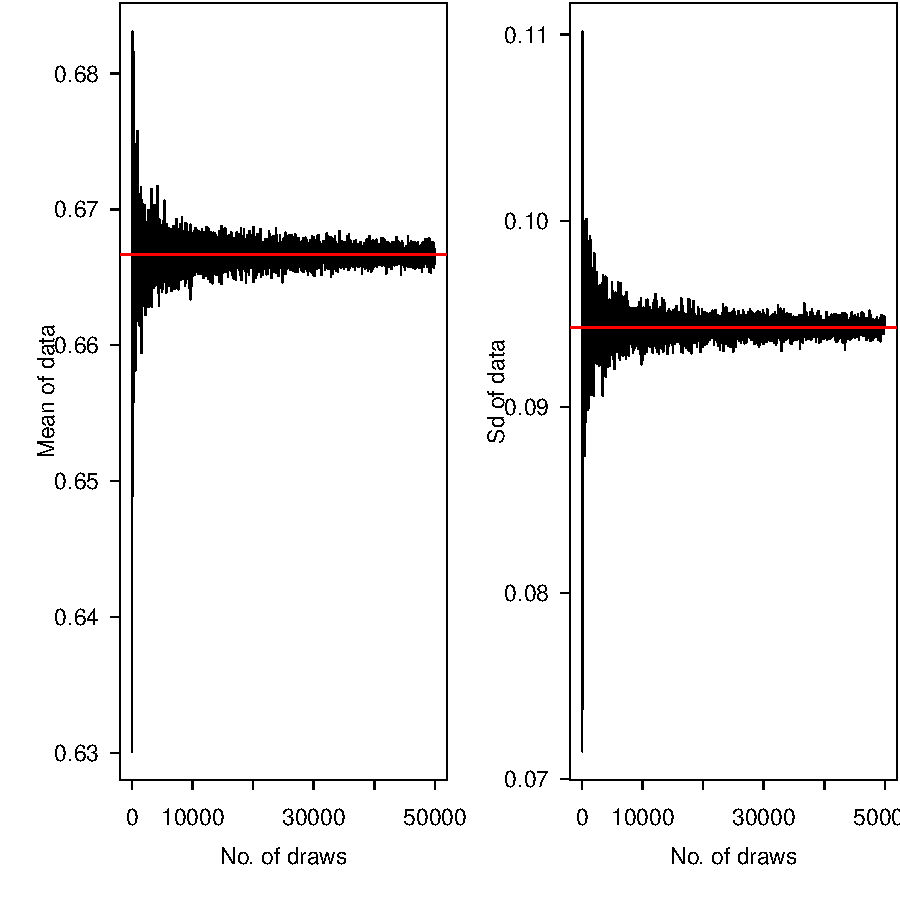
\includegraphics[width=.6\linewidth]{figure/lab1-Rnwauto-report-1} 

}


\begin{kframe}\begin{alltt}
\hlcom{# b) }
\hlcom{# Setup}
\hlstd{n} \hlkwb{=} \hlnum{20}
\hlstd{s} \hlkwb{=} \hlnum{14}
\hlstd{f} \hlkwb{=} \hlstd{n} \hlopt{-} \hlstd{s}
\hlstd{nDraws} \hlkwb{=} \hlnum{10000}

\hlcom{# Prior}
\hlstd{prior.alpha} \hlkwb{=} \hlnum{2}
\hlstd{prior.beta} \hlkwb{=} \hlnum{2}

\hlcom{# Posterior}
\hlstd{posterior.alpha} \hlkwb{<-} \hlstd{prior.alpha} \hlopt{+} \hlstd{s}
\hlstd{posterior.beta} \hlkwb{<-} \hlstd{prior.beta} \hlopt{+} \hlstd{f}
\hlstd{posterior.draws_means} \hlkwb{=} \hlkwd{numeric}\hlstd{()}
\hlstd{posterior.draws_sd} \hlkwb{=} \hlkwd{numeric}\hlstd{()}

\hlcom{# Draws}
\hlstd{posterior.draws_10000} \hlkwb{<-} \hlkwd{rbeta}\hlstd{(}\hlkwc{n} \hlstd{= nDraws,}
                               \hlkwc{shape1} \hlstd{= posterior.alpha,}
                               \hlkwc{shape2} \hlstd{= posterior.beta)}

\hlcom{# Calculate probability}
\hlstd{posterior.prob_0.4} \hlkwb{<-} \hlkwd{length}\hlstd{(}\hlkwd{which}\hlstd{(posterior.draws_10000} \hlopt{<} \hlnum{0.4}\hlstd{))}\hlopt{/}\hlkwd{length}\hlstd{(posterior.draws_10000)}
\hlstd{posterior.prob_real}\hlkwb{<-} \hlkwd{pbeta}\hlstd{(}\hlkwc{q} \hlstd{=} \hlnum{0.4}\hlstd{,}
                            \hlkwc{shape1} \hlstd{= posterior.alpha,}
                            \hlkwc{shape2} \hlstd{= posterior.beta)}

\hlcom{# c)}
\hlcom{# Functions}
\hlstd{logOdds} \hlkwb{<-} \hlkwa{function}\hlstd{(}\hlkwc{theta}\hlstd{) \{}
  \hlkwd{return} \hlstd{(}\hlkwd{log}\hlstd{(theta}\hlopt{/}\hlstd{(}\hlnum{1}\hlopt{-}\hlstd{theta)))}
\hlstd{\}}

\hlcom{# Setup}
\hlstd{n} \hlkwb{=} \hlnum{20}
\hlstd{s} \hlkwb{=} \hlnum{14}
\hlstd{f} \hlkwb{=} \hlstd{n} \hlopt{-} \hlstd{s}
\hlstd{nDraws} \hlkwb{=} \hlnum{10000}

\hlcom{# Prior}
\hlstd{prior.alpha} \hlkwb{=} \hlnum{2}
\hlstd{prior.beta} \hlkwb{=} \hlnum{2}

\hlcom{# Posterior}
\hlstd{posterior.alpha} \hlkwb{<-} \hlstd{prior.alpha} \hlopt{+} \hlstd{s}
\hlstd{posterior.beta} \hlkwb{<-} \hlstd{prior.beta} \hlopt{+} \hlstd{f}

\hlcom{# Draws}
\hlstd{posterior.draws_10000} \hlkwb{<-} \hlkwd{rbeta}\hlstd{(}\hlkwc{n} \hlstd{= nDraws,}
                               \hlkwc{shape1} \hlstd{= posterior.alpha,}
                               \hlkwc{shape2} \hlstd{= posterior.beta)}

\hlcom{# Log-odds the draws}
\hlstd{logOdds.draws} \hlkwb{<-}\hlkwd{logOdds}\hlstd{(posterior.draws_10000)}

\hlcom{# Hist and plot the density function of the log-odds draws}
\hlkwd{hist}\hlstd{(logOdds.draws,} \hlkwc{probability} \hlstd{=} \hlnum{TRUE}\hlstd{)}
\hlkwd{lines}\hlstd{(}\hlkwd{density}\hlstd{(logOdds.draws),} \hlkwc{col} \hlstd{=} \hlstr{'red'}\hlstd{)}

\hlcom{############# Task 2 #############}
\hlcom{# Log-normal distribution and the Gini coefficient}
\hlcom{# Likelihood: y_1, ..., y_n | µ, σ2 ~ log[ N(µ, σ2) ], µ known, σ2 unknown}
\hlcom{# Prior: p(σ2) ∝ 1/σ2}

\hlcom{# Posterior of σ2: Inv-X(n, tao^2)}
\hlcom{# Tao^2 - The sample variance. Calculated as following:}
\hlcom{# sum[ (log(y_i) - µ)^2 ]/n}

\hlcom{# If X ~ N(0, 1)}
\hlcom{# Y = exp(X) ~ log[ N(0,1) ] (lognormal)}

\hlcom{# Setup}
\hlstd{y} \hlkwb{<-} \hlkwd{c}\hlstd{(}\hlnum{14}\hlstd{,} \hlnum{25}\hlstd{,} \hlnum{45}\hlstd{,} \hlnum{25}\hlstd{,} \hlnum{30}\hlstd{,} \hlnum{33}\hlstd{,} \hlnum{19}\hlstd{,} \hlnum{50}\hlstd{,} \hlnum{34}\hlstd{,} \hlnum{67}\hlstd{)}
\hlstd{nDraws} \hlkwb{=} \hlnum{10000}
\hlstd{mu} \hlkwb{=} \hlnum{3.5}

\hlcom{# a)}
\hlcom{# Functions}
\hlstd{scaled_rchisq} \hlkwb{<-} \hlkwa{function}\hlstd{(}\hlkwc{Y}\hlstd{,} \hlkwc{mu}\hlstd{,} \hlkwc{nDraws}\hlstd{) \{}
  \hlstd{n} \hlkwb{<-} \hlkwd{length}\hlstd{(Y)} \hlcom{# Length of data}
  \hlstd{Z} \hlkwb{<-} \hlkwd{rchisq}\hlstd{(}\hlkwc{n} \hlstd{= nDraws,} \hlkwc{df} \hlstd{= n)} \hlcom{# Draw from Chi-squared distribution}
  \hlstd{tao2} \hlkwb{<-} \hlkwd{sum}\hlstd{((}\hlkwd{log}\hlstd{(Y)} \hlopt{-} \hlstd{mu)}\hlopt{^}\hlnum{2}\hlstd{)}\hlopt{/}\hlstd{n} \hlcom{# Calculate tau2 (sample standard diviation)}

  \hlkwd{return} \hlstd{(n}\hlopt{*}\hlstd{tao2}\hlopt{/}\hlstd{Z)}
\hlstd{\}}

\hlstd{σ2.draws} \hlkwb{<-} \hlkwd{scaled_rchisq}\hlstd{(y, mu, nDraws)} \hlcom{# Draw from Scaled inverse chi-squared distribution}
\hlkwd{hist}\hlstd{(σ2.draws,} \hlkwc{breaks}\hlstd{=}\hlnum{1000}\hlstd{)}
\end{alltt}


{\ttfamily\noindent\color{warningcolor}{\#\# Warning in title(main = main, sub = sub, xlab = xlab, ylab = ylab, ...): conversion failure on 'Histogram of σ2.draws' in 'mbcsToSbcs': dot substituted for <cf>}}

{\ttfamily\noindent\color{warningcolor}{\#\# Warning in title(main = main, sub = sub, xlab = xlab, ylab = ylab, ...): conversion failure on 'Histogram of σ2.draws' in 'mbcsToSbcs': dot substituted for <83>}}

{\ttfamily\noindent\color{warningcolor}{\#\# Warning in title(main = main, sub = sub, xlab = xlab, ylab = ylab, ...): conversion failure on 'σ2.draws' in 'mbcsToSbcs': dot substituted for <cf>}}

{\ttfamily\noindent\color{warningcolor}{\#\# Warning in title(main = main, sub = sub, xlab = xlab, ylab = ylab, ...): conversion failure on 'σ2.draws' in 'mbcsToSbcs': dot substituted for <83>}}\end{kframe}

{\centering 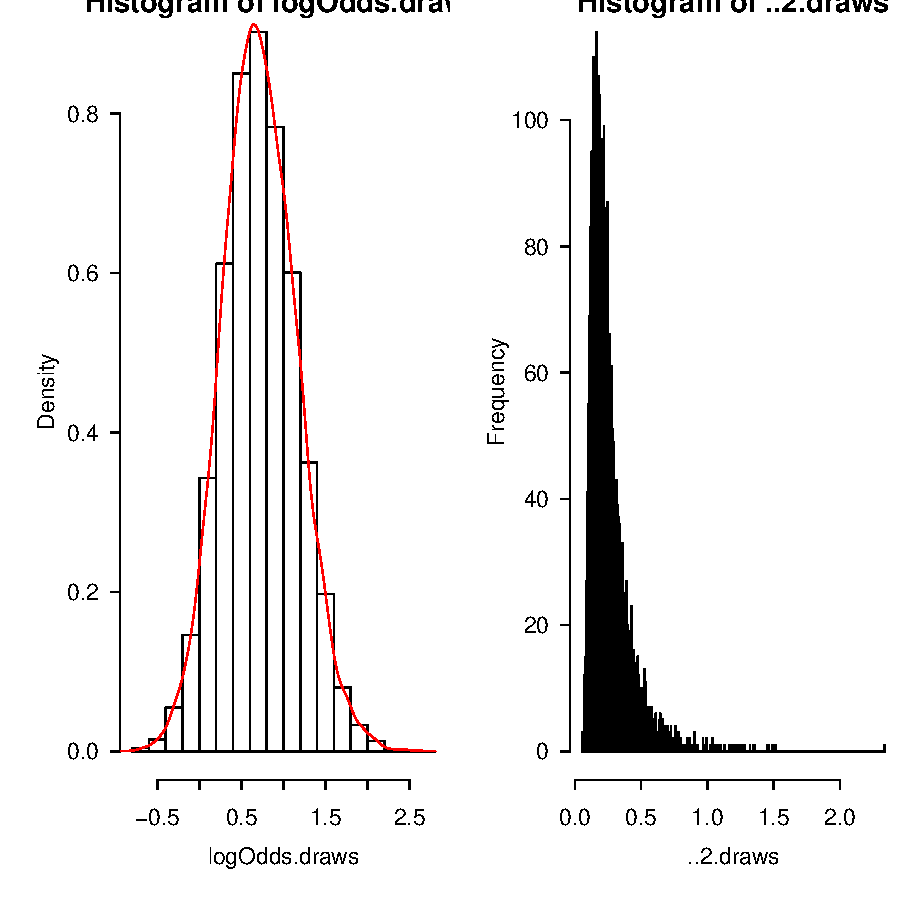
\includegraphics[width=.6\linewidth]{figure/lab1-Rnwauto-report-2} 

}


\begin{kframe}\begin{alltt}
\hlcom{# b)}
\hlcom{# Gini-coefficient measuers inequality (0: equal, 1: unequal)}
\hlcom{# Uses the Lorenz curve where:}
\hlcom{# x-axis: Cumulative share of people from low to high income}
\hlcom{# y-axis: Cumulative share of income earned}
\hlcom{#}
\hlcom{# If a straight line, it's 100% equal}
\hlcom{#}
\hlcom{# The Gini-coefficient is the ratio between the area between the straight line and the Lorenz curve}
\hlcom{# divided by the total area}
\hlcom{#}
\hlcom{# If the data follows an lognormal distribution (e.g wealth), the Gini-coef is calculated as follows:}
\hlcom{# G = 2 * Φ(σ/√2) - 1}

\hlstd{σ} \hlkwb{<-} \hlkwd{sqrt}\hlstd{(σ2.draws)} \hlcom{# Square σ2 to get σ}
\hlstd{gini_coef} \hlkwb{<-} \hlnum{2} \hlopt{*} \hlkwd{pnorm}\hlstd{(σ}\hlopt{/}\hlkwd{sqrt}\hlstd{(}\hlnum{2}\hlstd{),} \hlkwc{mean} \hlstd{=} \hlnum{0}\hlstd{,} \hlkwc{sd} \hlstd{=} \hlnum{1}\hlstd{)} \hlopt{-} \hlnum{1} \hlcom{# Calculate the Gini-coefficients for each σ}
\hlkwd{hist}\hlstd{(gini_coef,} \hlkwc{breaks}\hlstd{=}\hlnum{200}\hlstd{,} \hlkwc{probability} \hlstd{=} \hlnum{TRUE}\hlstd{)} \hlcom{# Hist Gini-coefficients}
\hlkwd{lines}\hlstd{(}\hlkwd{density}\hlstd{(gini_coef),} \hlkwc{col}\hlstd{=}\hlstr{'red'}\hlstd{)} \hlcom{# Plot density curve}

\hlcom{# c)}
\hlcom{# Functions}
\hlstd{eqtail_CI} \hlkwb{<-} \hlkwa{function}\hlstd{(}\hlkwc{..X}\hlstd{,} \hlkwc{interval}\hlstd{) \{}
  \hlstd{lower} \hlkwb{<-} \hlstd{(}\hlnum{1}\hlopt{-}\hlstd{interval)}\hlopt{/}\hlnum{2}
  \hlstd{upper} \hlkwb{<-} \hlnum{1} \hlopt{-} \hlstd{lower}
  \hlstd{n} \hlkwb{<-} \hlkwd{length}\hlstd{(..X)}
  \hlstd{X} \hlkwb{<-} \hlkwd{sort}\hlstd{(..X)} \hlcom{# Sort from smallest to largest value}

  \hlkwd{return} \hlstd{(}\hlkwd{list}\hlstd{(}\hlkwc{lower}\hlstd{=X[n}\hlopt{*}\hlstd{lower],} \hlkwc{upper}\hlstd{=X[n}\hlopt{*}\hlstd{upper]))}
\hlstd{\}}

\hlstd{HPD} \hlkwb{<-} \hlkwa{function}\hlstd{(}\hlkwc{density}\hlstd{,} \hlkwc{interval}\hlstd{) \{}
  \hlstd{gini_df} \hlkwb{<-} \hlkwd{data.frame}\hlstd{(}\hlkwc{x} \hlstd{= density}\hlopt{$}\hlstd{x,} \hlkwc{y} \hlstd{= density}\hlopt{$}\hlstd{y)}
  \hlstd{gini_df} \hlkwb{<-} \hlstd{gini_df[}\hlkwd{with}\hlstd{(gini_df,} \hlkwd{order}\hlstd{(y)),]}
  \hlstd{gini_df} \hlkwb{<-} \hlkwd{data.frame}\hlstd{(}\hlkwc{x} \hlstd{= gini_df}\hlopt{$}\hlstd{x,} \hlkwc{y} \hlstd{= gini_df}\hlopt{$}\hlstd{y)}
  \hlstd{n} \hlkwb{<-} \hlkwd{dim}\hlstd{(gini_df)[}\hlnum{1}\hlstd{]}
  \hlstd{lower} \hlkwb{<-} \hlnum{1} \hlopt{-} \hlstd{interval}
  \hlkwd{print}\hlstd{(lower)}
  \hlstd{HPD_cumsum} \hlkwb{<-} \hlkwd{cumsum}\hlstd{(gini_df}\hlopt{$}\hlstd{y)}\hlopt{/}\hlkwd{sum}\hlstd{(gini_df}\hlopt{$}\hlstd{y)}
  \hlstd{HPD_lower} \hlkwb{<-} \hlkwd{which}\hlstd{(HPD_cumsum} \hlopt{>=} \hlstd{lower)[}\hlnum{1}\hlstd{]}
  \hlstd{gini_df_95} \hlkwb{<-} \hlstd{gini_df[(HPD_lower} \hlopt{+} \hlnum{1}\hlstd{)}\hlopt{:}\hlstd{n, ]}
  \hlstd{HPD_interval} \hlkwb{<-} \hlkwd{c}\hlstd{(}\hlkwd{min}\hlstd{(gini_df_95}\hlopt{$}\hlstd{x),} \hlkwd{max}\hlstd{(gini_df_95}\hlopt{$}\hlstd{x))}
  \hlkwd{return} \hlstd{(}\hlkwd{list}\hlstd{(}\hlkwc{lower} \hlstd{= HPD_interval[}\hlnum{1}\hlstd{],} \hlkwc{upper} \hlstd{= HPD_interval[}\hlnum{2}\hlstd{]))}
\hlstd{\}}

\hlcom{# 95% equal tail credible interval}
\hlstd{gini_coef_CI} \hlkwb{<-} \hlkwd{eqtail_CI}\hlstd{(gini_coef,} \hlnum{0.95}\hlstd{)}

\hlkwd{hist}\hlstd{(gini_coef,} \hlkwc{breaks}\hlstd{=}\hlnum{200}\hlstd{,} \hlkwc{probability} \hlstd{=} \hlnum{TRUE}\hlstd{)} \hlcom{# Hist Gini-coefficients}
\hlkwd{lines}\hlstd{(}\hlkwd{density}\hlstd{(gini_coef),} \hlkwc{col}\hlstd{=}\hlstr{'red'}\hlstd{)} \hlcom{# Plot density curve}
\hlkwd{abline}\hlstd{(}\hlkwc{v} \hlstd{= gini_coef_CI}\hlopt{$}\hlstd{lower,} \hlkwc{col}\hlstd{=}\hlstr{'blue'}\hlstd{)} \hlcom{# Plot lower CI line}
\hlkwd{abline}\hlstd{(}\hlkwc{v} \hlstd{= gini_coef_CI}\hlopt{$}\hlstd{upper,} \hlkwc{col}\hlstd{=}\hlstr{'blue'}\hlstd{)} \hlcom{# Plot upper CI line}
\end{alltt}
\end{kframe}

{\centering 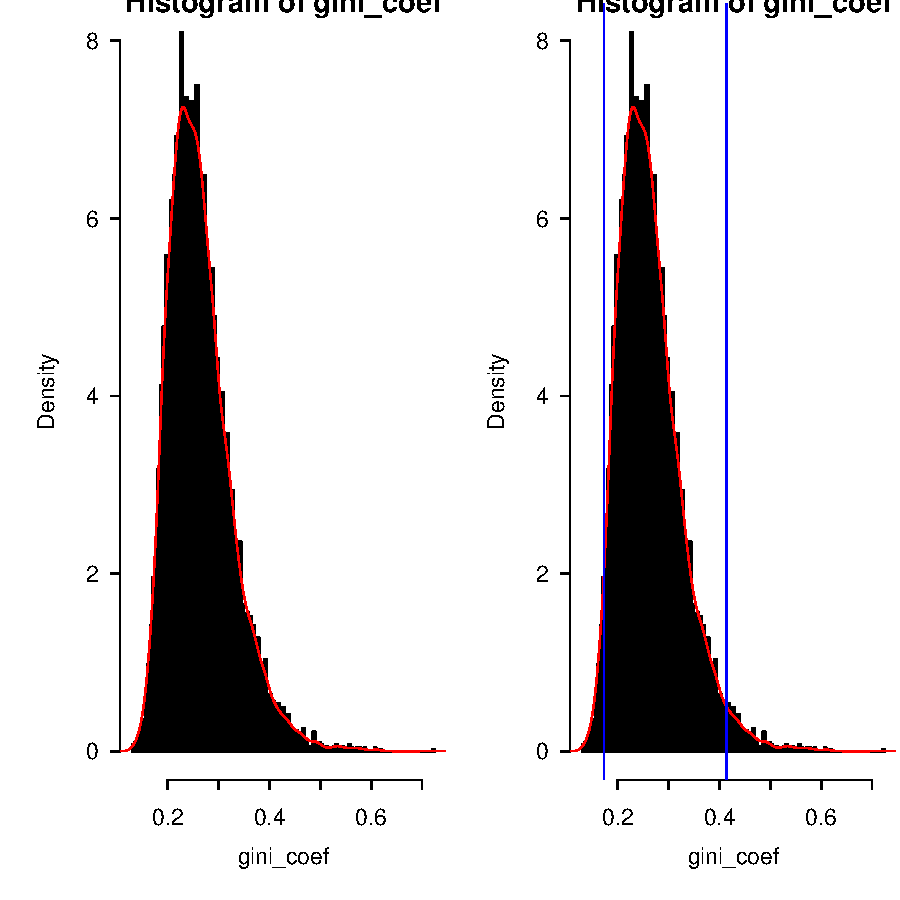
\includegraphics[width=.6\linewidth]{figure/lab1-Rnwauto-report-3} 

}


\begin{kframe}\begin{alltt}
\hlcom{# Highest Posterior Density Interval}
\hlstd{gini_density} \hlkwb{<-} \hlkwd{density}\hlstd{(gini_coef)}
\hlstd{HPD_interval} \hlkwb{<-} \hlkwd{HPD}\hlstd{(gini_density,} \hlnum{0.95}\hlstd{)}
\end{alltt}
\begin{verbatim}
## [1] 0.05
\end{verbatim}
\begin{alltt}
\hlcom{# Plot histogram of Gini coefficients, 95% credible interval (blue) and 95% HPD interval (green)}
\hlkwd{hist}\hlstd{(gini_coef,} \hlkwc{breaks}\hlstd{=}\hlnum{200}\hlstd{,} \hlkwc{probability} \hlstd{=} \hlnum{TRUE}\hlstd{)} \hlcom{# Hist Gini-coefficients}
\hlkwd{lines}\hlstd{(}\hlkwd{density}\hlstd{(gini_coef),} \hlkwc{col}\hlstd{=}\hlstr{'red'}\hlstd{)} \hlcom{# Plot density curve}
\hlkwd{abline}\hlstd{(}\hlkwc{v} \hlstd{= gini_coef_CI}\hlopt{$}\hlstd{lower,} \hlkwc{col}\hlstd{=}\hlstr{'blue'}\hlstd{)} \hlcom{# Plot lower CI line}
\hlkwd{abline}\hlstd{(}\hlkwc{v} \hlstd{= gini_coef_CI}\hlopt{$}\hlstd{upper,} \hlkwc{col}\hlstd{=}\hlstr{'blue'}\hlstd{)} \hlcom{# Plot upper CI line}
\hlkwd{abline}\hlstd{(}\hlkwc{v} \hlstd{= HPD_interval}\hlopt{$}\hlstd{lower,} \hlkwc{col}\hlstd{=}\hlstr{'green'}\hlstd{)} \hlcom{# Plot lower HPD interval}
\hlkwd{abline}\hlstd{(}\hlkwc{v} \hlstd{= HPD_interval}\hlopt{$}\hlstd{upper,} \hlkwc{col}\hlstd{=}\hlstr{'green'}\hlstd{)} \hlcom{# Plot upper HPD interval}

\hlcom{############# Task 3 #############}
\hlcom{# von Mises distribution looks like a normal distribution with a spiky top and}
\hlcom{# is a continues probability distribution on the circle, where theta is an angle.}
\hlcom{# Kappa (κ): Concentration parameter. Large κ gives small variance around µ.}
\hlcom{# Likelihood: p(y_1, ..., y_n | µ, κ) = exp[ κ * cos(y - µ) ]/(2πIo(κ))}
\hlcom{# Prior: κ ~ Exp(λ = 1), mean = 1/λ}

\hlcom{# Setup}
\hlcom{# Wind-angles in degrees on 10 different days}
\hlcom{# North is zero}
\hlcom{# }
\hlstd{y.degrees} \hlkwb{<-} \hlkwd{c}\hlstd{(}\hlnum{40}\hlstd{,} \hlnum{303}\hlstd{,} \hlnum{326}\hlstd{,} \hlnum{285}\hlstd{,} \hlnum{296}\hlstd{,} \hlnum{314}\hlstd{,} \hlnum{20}\hlstd{,} \hlnum{308}\hlstd{,} \hlnum{299}\hlstd{,} \hlnum{296}\hlstd{)}
\hlstd{y.radians} \hlkwb{<-} \hlkwd{c}\hlstd{(}\hlopt{-}\hlnum{2.44}\hlstd{,} \hlnum{2.14}\hlstd{,} \hlnum{2.54}\hlstd{,} \hlnum{1.83}\hlstd{,} \hlnum{2.02}\hlstd{,} \hlnum{2.33}\hlstd{,} \hlopt{-}\hlnum{2.79}\hlstd{,} \hlnum{2.23}\hlstd{,} \hlnum{2.07}\hlstd{,} \hlnum{2.02}\hlstd{)}
\hlstd{mu} \hlkwb{<-} \hlnum{2.39} \hlcom{# Mean directon}

\hlcom{# a)}
\hlcom{# Prior}
\hlstd{kappa} \hlkwb{<-} \hlkwd{data.frame}\hlstd{(}\hlkwc{seq} \hlstd{=} \hlkwd{seq}\hlstd{(}\hlnum{0}\hlstd{,} \hlnum{10}\hlstd{,} \hlnum{0.01}\hlstd{),}
                    \hlkwc{posterior} \hlstd{=} \hlnum{0}
\hlstd{)}

\hlkwa{for} \hlstd{(i} \hlkwa{in} \hlnum{1}\hlopt{:}\hlkwd{dim}\hlstd{(kappa)[}\hlnum{1}\hlstd{]) \{} \hlcom{# Loop over every kappa}
  \hlstd{k} \hlkwb{<-} \hlstd{kappa}\hlopt{$}\hlstd{seq[i]} \hlcom{# Extract current kappa}
  \hlstd{prior} \hlkwb{<-} \hlkwd{exp}\hlstd{(}\hlopt{-}\hlstd{k)} \hlcom{# Calculate prior with current kappa}
  \hlstd{bessel} \hlkwb{<-} \hlkwd{besselI}\hlstd{(}\hlkwc{x} \hlstd{= k,}
                    \hlkwc{nu} \hlstd{=} \hlnum{0}\hlstd{)} \hlcom{# Bessel-function}
  \hlstd{likelihood} \hlkwb{<-} \hlkwd{prod}\hlstd{(}\hlkwd{exp}\hlstd{(k} \hlopt{*} \hlkwd{cos}\hlstd{(y.radians} \hlopt{-} \hlstd{mu))}\hlopt{/}\hlstd{(}\hlnum{2}\hlopt{*}\hlstd{pi}\hlopt{*}\hlstd{bessel))} \hlcom{# Calculate von Mises probability}
  \hlstd{kappa}\hlopt{$}\hlstd{posterior[i]} \hlkwb{<-} \hlstd{likelihood} \hlopt{*} \hlstd{prior} \hlcom{# Calculate posterior with current kappa}
\hlstd{\}}

\hlcom{# Plot posterior for different kappas}
\hlkwd{plot}\hlstd{(kappa}\hlopt{$}\hlstd{seq, kappa}\hlopt{$}\hlstd{posterior,} \hlkwc{type}\hlstd{=}\hlstr{'l'}\hlstd{)}
\end{alltt}
\end{kframe}

{\centering 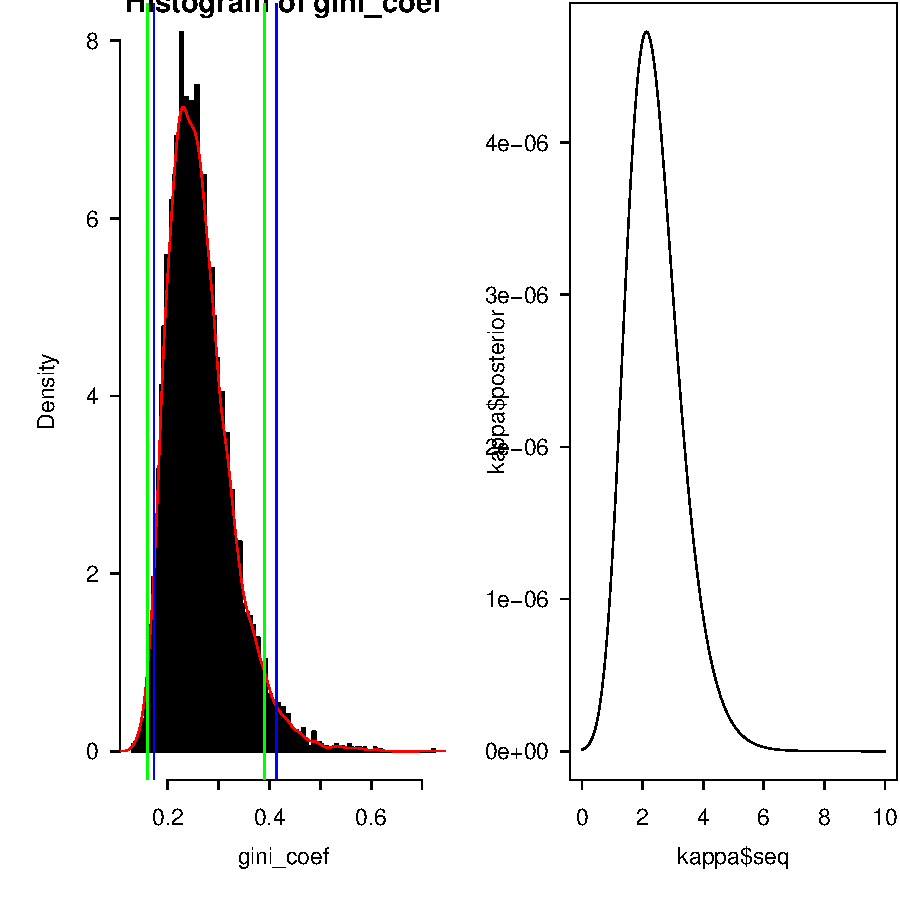
\includegraphics[width=.6\linewidth]{figure/lab1-Rnwauto-report-4} 

}


\begin{kframe}\begin{alltt}
\hlcom{# b)}
\hlstd{index} \hlkwb{<-} \hlkwd{which.max}\hlstd{(kappa}\hlopt{$}\hlstd{posterior)} \hlcom{# Finds index with maximum posterior}
\hlstd{kappa.mode} \hlkwb{<-} \hlstd{kappa}\hlopt{$}\hlstd{seq[}\hlkwd{which.max}\hlstd{(kappa}\hlopt{$}\hlstd{posterior)]} \hlcom{# Extract kappa with maximum posterior}

\hlkwd{plot}\hlstd{(kappa}\hlopt{$}\hlstd{seq, kappa}\hlopt{$}\hlstd{posterior,} \hlkwc{type}\hlstd{=}\hlstr{'l'}\hlstd{)}
\hlkwd{abline}\hlstd{(}\hlkwc{v} \hlstd{= kappa.mode,} \hlkwc{col}\hlstd{=}\hlstr{'red'}\hlstd{)}
\end{alltt}
\end{kframe}

{\centering 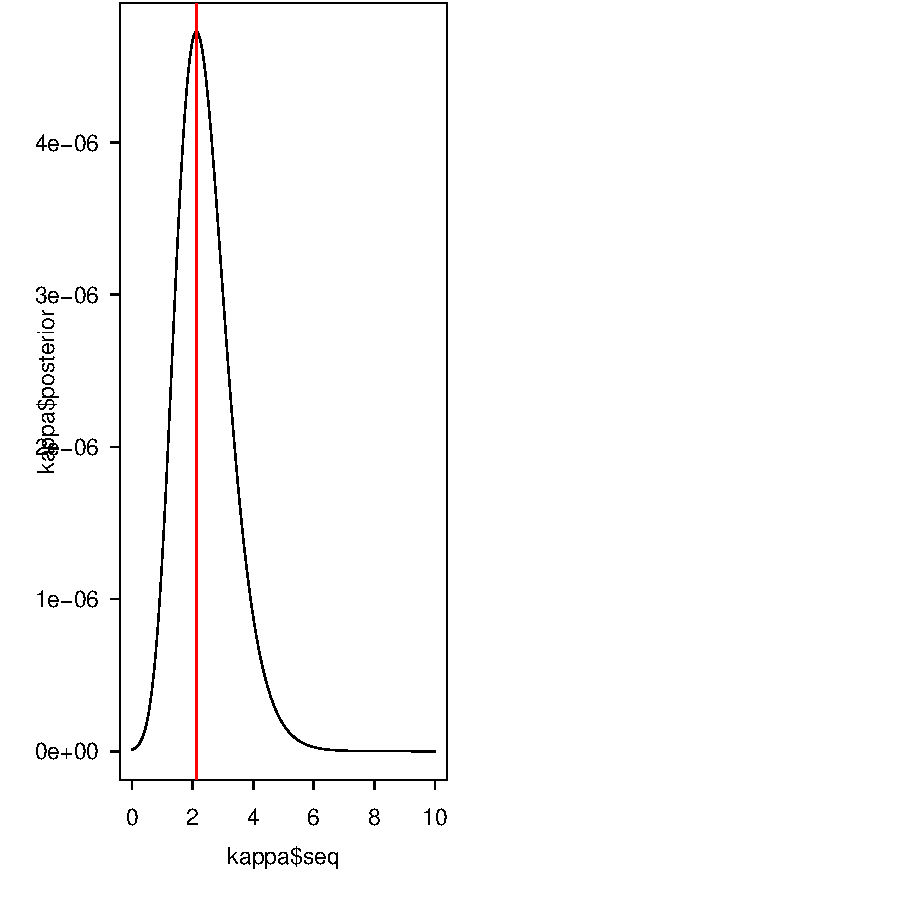
\includegraphics[width=.6\linewidth]{figure/lab1-Rnwauto-report-5} 

}



\end{knitrout}

The R session information (including the OS info, R version and all
packages used):

\begin{knitrout}
\definecolor{shadecolor}{rgb}{0.969, 0.969, 0.969}\color{fgcolor}\begin{kframe}
\begin{alltt}
\hlkwd{sessionInfo}\hlstd{()}
\end{alltt}
\begin{verbatim}
## R version 3.4.2 (2017-09-28)
## Platform: x86_64-apple-darwin15.6.0 (64-bit)
## Running under: OS X El Capitan 10.11.6
## 
## Matrix products: default
## BLAS: /System/Library/Frameworks/Accelerate.framework/Versions/A/Frameworks/vecLib.framework/Versions/A/libBLAS.dylib
## LAPACK: /System/Library/Frameworks/Accelerate.framework/Versions/A/Frameworks/vecLib.framework/Versions/A/libLAPACK.dylib
## 
## locale:
## [1] en_US.UTF-8/en_US.UTF-8/en_US.UTF-8/C/en_US.UTF-8/en_US.UTF-8
## 
## attached base packages:
## [1] stats     graphics  grDevices utils     datasets  methods   base     
## 
## other attached packages:
## [1] knitr_1.18         mvtnorm_1.0-7      rstan_2.17.3       StanHeaders_2.17.2
## [5] ggplot2_2.2.1     
## 
## loaded via a namespace (and not attached):
##  [1] Rcpp_0.12.13     codetools_0.2-15 grid_3.4.2       plyr_1.8.4       gtable_0.2.0    
##  [6] magrittr_1.5     stats4_3.4.2     evaluate_0.10.1  scales_0.5.0     highr_0.6       
## [11] stringi_1.1.5    rlang_0.1.4      lazyeval_0.2.1   tools_3.4.2      stringr_1.2.0   
## [16] munsell_0.4.3    yaml_2.1.16      compiler_3.4.2   inline_0.3.14    colorspace_1.3-2
## [21] gridExtra_2.3    tibble_1.3.4
\end{verbatim}
\begin{alltt}
\hlkwd{Sys.time}\hlstd{()}
\end{alltt}
\begin{verbatim}
## [1] "2018-05-28 15:50:33 CEST"
\end{verbatim}
\end{kframe}
\end{knitrout}


\end{document}
